The \lascar (LASer CAlibration Rod) card (Fig. \ref{fig:laslascar}) is a masterpiece of the \lasii~electronics scheme. This innovative board aims at controlling the \las~system with the following components:
\begin{itemize}

\item digitization through a charge analog-to-digital converter (QDC),

\item charge injection (LILAS) to monitor the stability of the electronics (photodiode preamplifiers+digitization),

\item time-to-digital converter (TDC) to estimate the time response of the \las~as a function of its intensity,

\item TTCRX : chip used to retrieve LHC signals,

\item HOLA card : sends data fragments,

\item \laser~interface : to drive the \las~(power, trigger).

\end{itemize}

\begin{figure}[htbp]

\centering
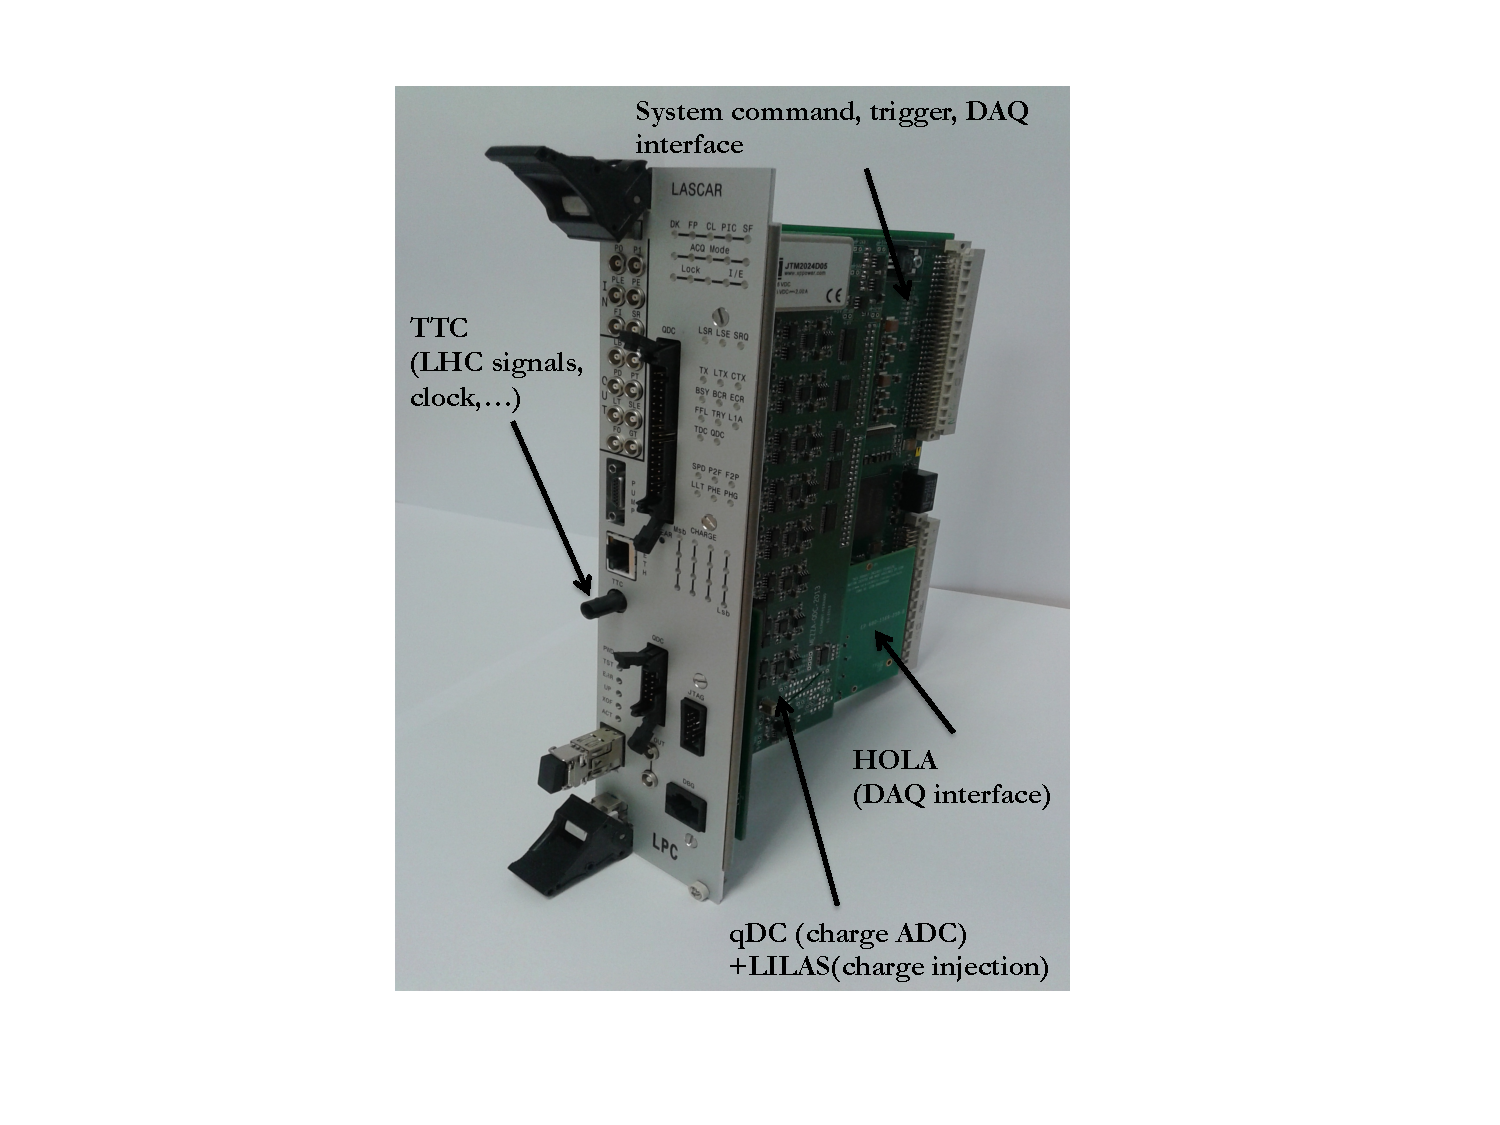
\includegraphics[height=10cm,width=11cm]{figures/Lascar_photo_black.pdf}
\includegraphics[height=9cm,width=5cm]{figures/Lascar_Cote.pdf}
\caption{Views of the \lascar~card}\label{fig:laslascar}
\end{figure}

The \lascar~card is housed in a VME crate and its adress is in the format A32/D32. The heart is composed of an Field Programmable Gate Array (FPGA) Cyclone V manufactured by ALTERA \cite{ref:altera-cyclone}.

The following inputs-outputs (Fig. \ref{fig:laslascarlinks}) are available :
\begin{itemize}
\item 16 analogic channels (differential mode) for the QDC,
\item 4 digital entries (NIM format),
\item 2 analogic entries for the photomultipliers,
\item 8 digital outputs (NIM format),
\item 1 analogic-digital interface with the \las,
\item one fiber (entry) to get information from the TTC,
\item one fiber (input-output) for acquisition,
\item one ethernet link for the DCS,
\item one interface with the VME bus,
\item one JTAG interface to configure the FPGA.

\end{itemize}

\begin{figure}[htbp]

\centering
\includegraphics[height=15cm,width=15cm]{figures/Lascarlinks.pdf}
\caption{Scheme of the \lascar~card}\label{fig:laslascarlinks}
\end{figure}


\paragraph{QDC}

The QDC of the \lascar~module (Fig. \ref{fig:laslascarqdc}) comprises 32 channels, each with a 14-bit, high speed, low power, successive approximation ADC that operates from a single 2.5 V power supply and features throughput rates of up to 4.2 MSPS. Each channel contains two ADCs, each preceded by a low noise, wide bandwidth track-and-hold circuit that can handle input frequencies in excess of 110 MHz. This part is preceded by two charge amplifiers with different slopes (x1 and x4). The analog signal at the entrance of the QDC is integrated during 500 ns (value adjustable through a VME register) and the maximum charge that may be integrated is of ~2000 pC. Analog signals that are to be converted arise from the eleven photodiodes, the two PMTs, and from the charge injection system (3 channels, one internal to the QDC, and 2 from the photodiode box). 
 
\begin{figure}[htbp]

\centering
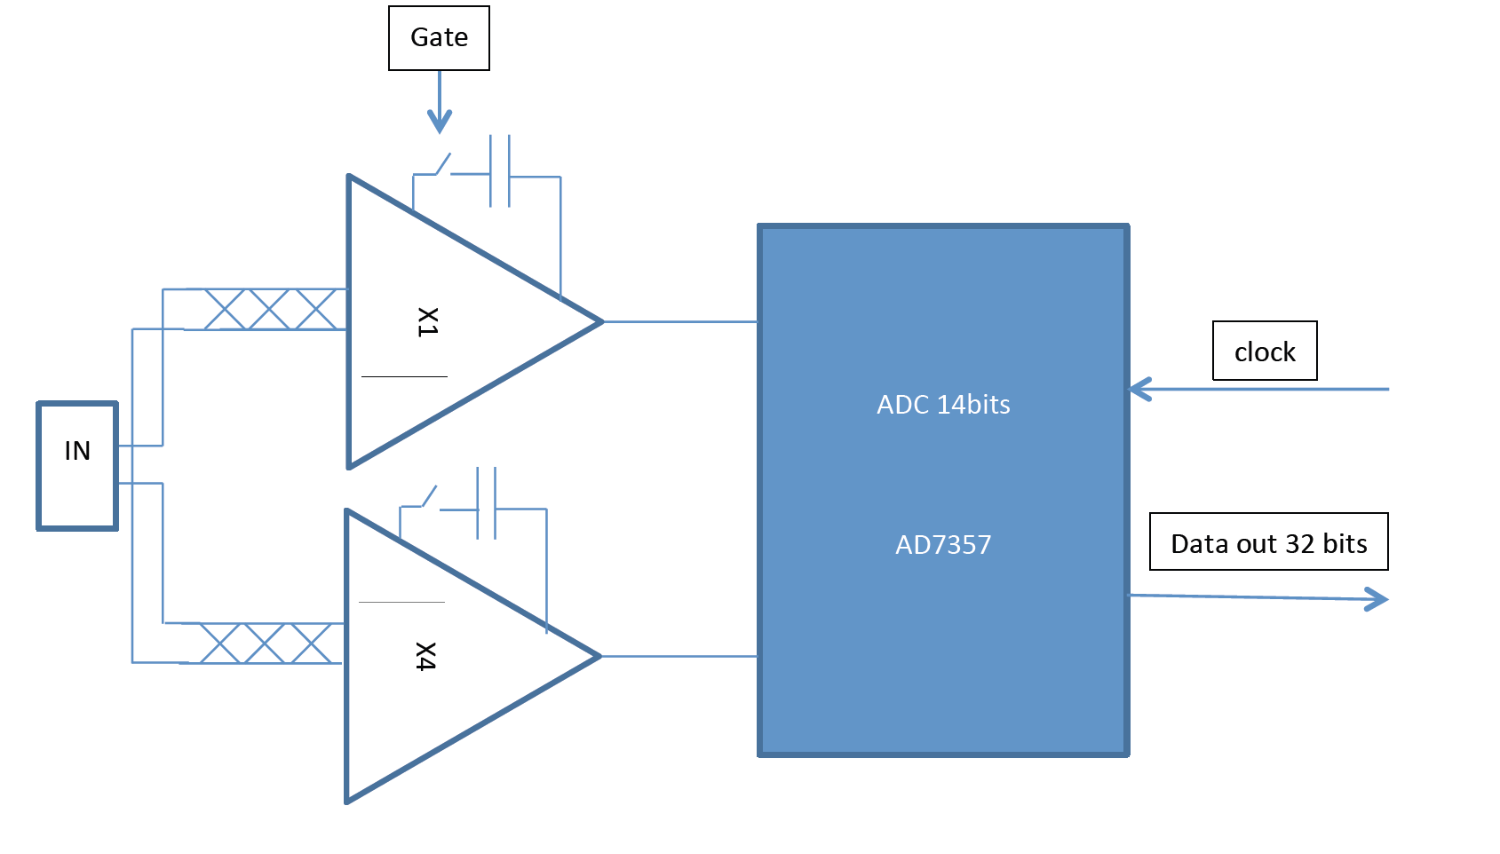
\includegraphics[height=5cm]{figures/qdc.pdf}
\caption{Scheme of the \lascar~QDC}\label{fig:laslascarqdc}
\end{figure}

\paragraph{LILAS}
The LILAS part of \lascar~(Fig. \ref{fig:laslascarlilas}) aims at injecting a known charge in each photodiode preamplifier so as to survey the linearity and the stability of the electronics with time. The charge is injected in the system through three ways : a direct link to one of the QDC channels (since the QDC and LILAS are located on the same printed board), and via two lemo cables plugged in the photodiode box and in \phocal.  

\begin{figure}[htbp]

\centering
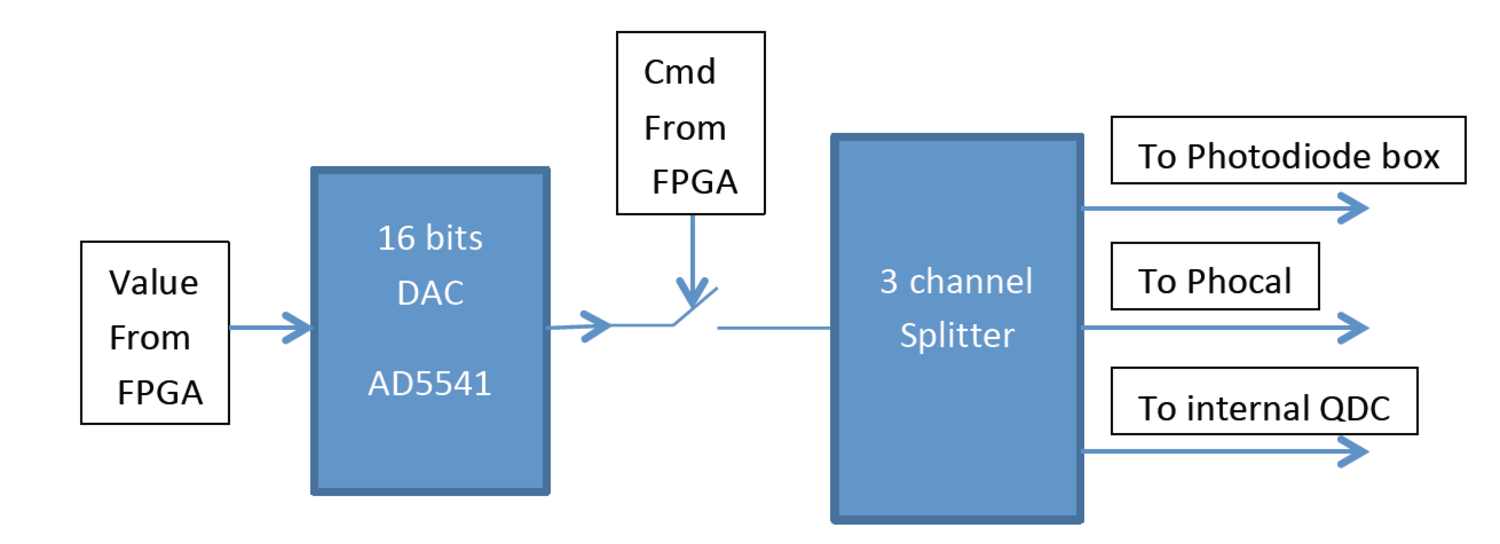
\includegraphics[height=3cm]{figures/lilas.pdf}
\caption{Scheme of the \lascar~LILAS}\label{fig:laslascarlilas}
\end{figure}

\paragraph{TDC}
The \lascar~TDC (Fig. \ref{fig:laslascartdc}) is a TDC-GP1, an integrated device manufactured by ACAM \cite{ref:tdc}. It contains two measuring channels with a typical resolution of 280 ps. This TDC aims at measuring the \las~time response as a function of its power. The time response as a function of the intensity has been measured for the \las~(J40-BL6S) we are using (Fig. \ref{fig:lasresponse}). Values around 420 ps are observed for lower intensities and a decrease to 320 ps is seen for higher intensities. The \lascar~card is equipped with a delay system so as to to send the \las~light in an "empty" bunch-crossing in a coherent way during the physics runs of the LHC.

\begin{figure}[htbp]

\centering
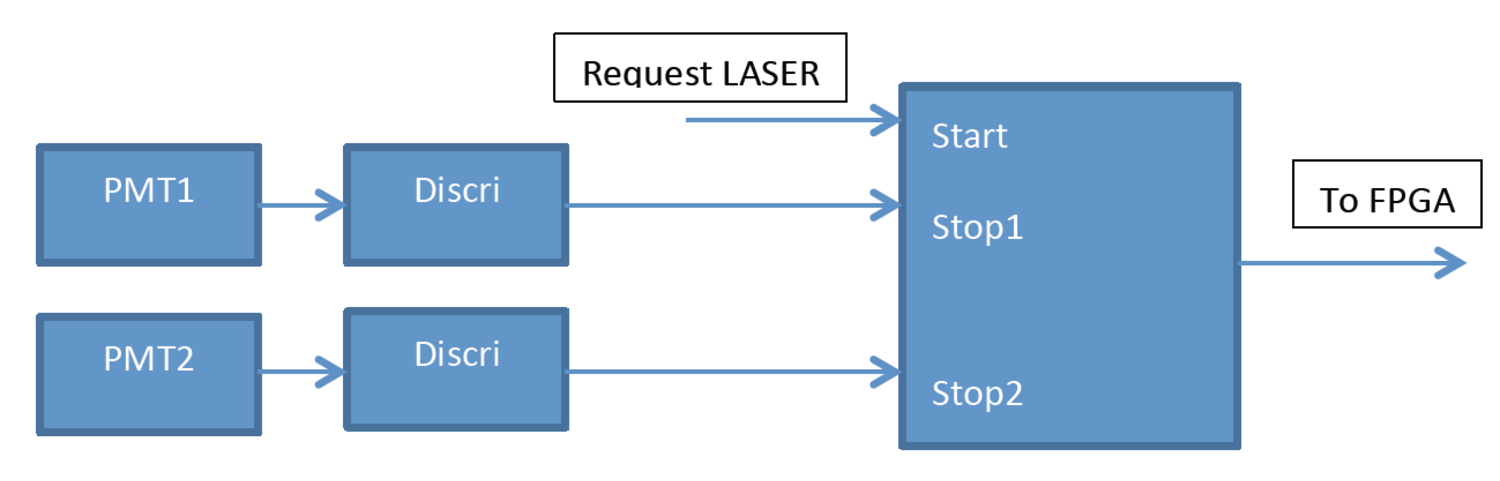
\includegraphics[height=3cm]{figures/tdc.pdf}
\caption{Scheme of the \lascar~TDC}\label{fig:laslascartdc}
\end{figure}

\paragraph{TTCRX}

The TTCRX \cite{ref:ttcrx} is an integrated circuit developped at CERN that retrieves the following LHC signals :
\begin{itemize}
\item Bunch Crossing (BC),
\item Bunch Crossing Reset (BCR),
\item Event Counter Reset (ECR),
\item Level one Accept (L1A),
\item Level one Identity (L1AID).
\end{itemize}

The FPGA will process these data prior to  a transmission to the TDAQ.

\begin{figure}[htbp]
\centering
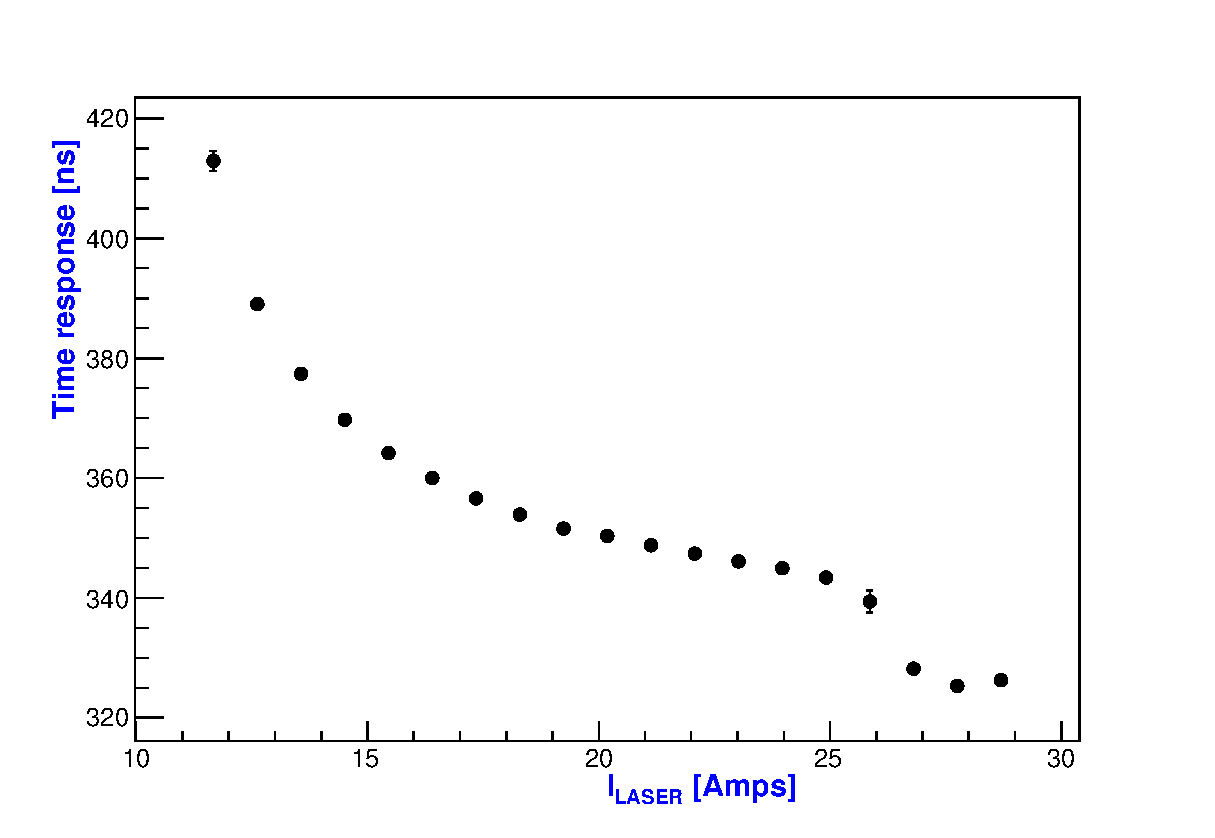
\includegraphics[height=5cm]{figures/laser_timing_new.eps}
\caption{\las~time response as a function of the intensity.}\label{fig:lasresponse}
\end{figure}


\paragraph{HOLA}

The HOLA card \cite{ref:hola} (Fig. \ref{fig:laslascarhola}) has been developed at CERN and is mounted on \lascar. It is used to send data fragments to the Read Out Buffer (ROB) via an optical fiber for each L1A.
\begin{figure}[htbp]

\centering
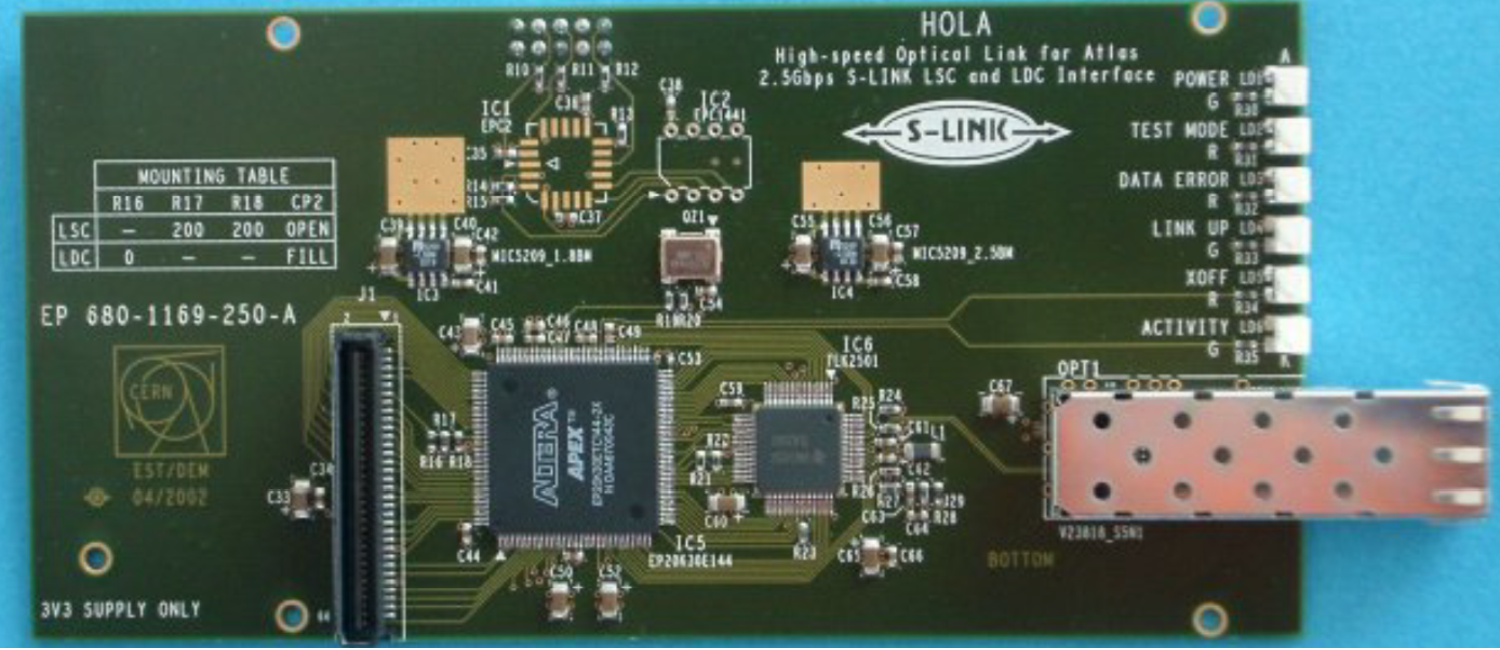
\includegraphics[height=5cm]{figures/hola.pdf}
\caption{View of the \lascar~HOLA}\label{fig:laslascarhola}
\end{figure}

\paragraph{LASER interface}

This mixed interface (analog and digital) (Fig. \ref{fig:laslaserint}) is used to control the \laser~J40-BL6S. The \laser~intensity is set with an analog voltage (from 0 to 4V) and the trigger part is done through a TTL signal.

\begin{figure}[htbp]

\centering
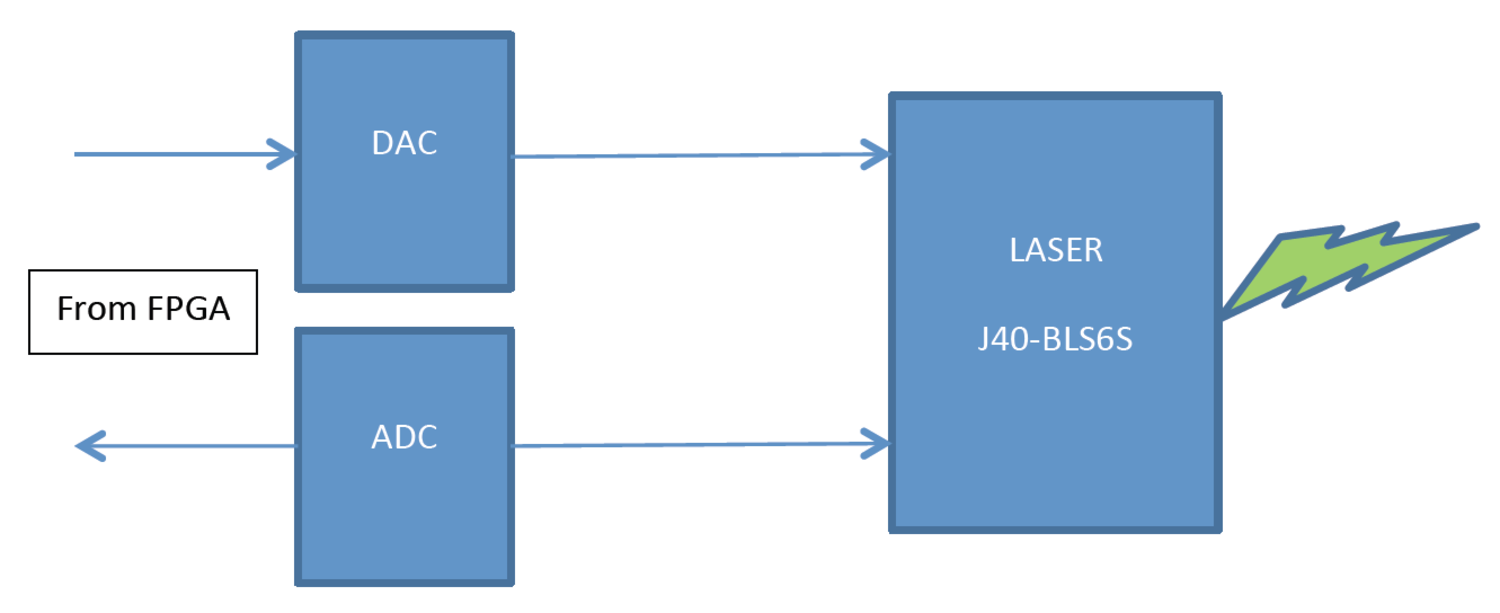
\includegraphics[height=3cm]{figures/laser_interface.pdf}
\caption{Scheme of the \lascar~\las~interface}\label{fig:laslaserint}
\end{figure}

\paragraph{Acquisition modes}

There are two independent ways of running the \laser~system : the stand-alone mode and the "ATLAS TDAQ" mode.

\begin{itemize}

\item Stand-alone mode

The stand-alone mode may be used to check that the \laser~system is responding as expected. Reference runs may be performed so as to monitor the stability of the system. The control interface of the QDC and of the TDC is done with the VME bus and the running frequency reaches about 100 Hz. The following possible modes are:
\begin{itemize}

\item Pedestal : to measure of the QDC output distributions when no input signal is injected. Pedestal values are subtracted when results from other modes (Alpha, LED, Linearity, LASER) are studied,

\item Alpha : to estimate the response of the reference (PHOCAL) photodiode to alpha particles emitted by the Americium source,

\item LED : the LED signal is transmitted to all the photodiodes via optical fibers. In this mode  the stability of the ten photodiodes used to monitor the \laser~light may be surveyed,

\item Linearity : a known charge is injected in the preamplifiers of the photodiodes so as to estimate the linearity and the stability of the electronics,

\item Laser: \laser~signals with varying intensities are sent in the system. The light may or may not be transmitted to the TileCal PMTs, depending on the status of the shutter located inside the optics box.

\end{itemize}

The way the acquisition is triggered for these modes are summarized in Tab. \ref{tab:lascargates}.

\begin{table}[htbp]
  \begin{center}
    \caption{Gate acquisition origin as a function of the running mode.}\label{tab:lascargates}
    \begin{tabular}{ll}
      \hline\hline
      Mode & Gate trigger \\
      \hline
      Pedestal & VME register \\
      Alpha & \phocal~discriminator\\
      LED & \phocal~pulse \\
	Linearity & VME register \\
      \laser & PMT1 and PMT2 signal \\
      \hline
    \end{tabular}
  \end{center}
\end{table}

Raw data are stored as Trees of the ROOT \cite{ref:root} Data Analysis Framework. For each event (i.e. each time a gate is open), the date, the number of QDC counts for each photodiode and each gain (32 words), the TDC values, the order (filled in case of a \laser~run or for the linearity mode) are information that may be used for analysis. 

It is possible to run the stand-alone mode through a GUI interface developed with ROOT tools as illustrated by Fig. \ref{fig:lasstandgui} in \ref{app}. For each type of run, it is possible to choose the run conditions (number of events, shutter state, intensity of the \laser, filter wheel position, ...). A display of the results (histograms) is automatically performed when the run has ended.

\item ATLAS TDAQ mode

This mode is used in two ways: twice a week when calibration runs are performed and during physics runs, when \laser~pulses are emitted in empty bunch-crossings (every second). The control interface is provided by the SHAFT electronic module which sends requests to \lascar. Output data fragments are transmitted via the HOLA card for each L1A and \laser~Trigger Type.

The modes available are the same as in stand-alone : Pedestal, Alpha, LED, Linearity, Laser. One possibility has been added. The "combined" mode consists in running Pedestal, LED and Alpha modes in a row. For each mode, the sum of the output values and of their squares are calculated and stored in a RAM. These values are then trasmitted in a data fragment (through the HOLA card for each L1A and \laser~Trigger Type) when the \laser~mode is activated.

Two kinds of data fragments may be transmitted, depending on the DAQ mode selected (see section \ref{sec:daq}): a short one, used in the LaserCalib (Pedestal+Alpha+LED+Linearity) or LaserAlpha modes , and a long one, used in the Laser mode (\laser~light injected in the PMTs of the TileCal). Each fragment is composed of a header and of a data fragment (see Figs. \ref{fig:shortfrag}-\ref{fig:longfragb} in \ref{app}). Information such as the Daq type (Pedestal, LED, Alpha, Linearity, Laser), number of events, \laser~or charge intensity, raw QDC values of the photodiodes, TDC values, are stored in the short data fragment. The long data fragment contains the same information (but for the \laser~only) and is completed by the sum of the output values ($\Sigma$X) of the photodiodes (and of their squares $\Sigma$X$^{2}$) (for each QDC channel) of the most recent pedestal, alpha and LED runs. These data are transmitted in a sequential way. 

\end{itemize}
